\section{订单自预测型生产计划制订(问题四)} % (fold)
\label{sec:_问题四_}

\subsection{模型的建立} % (fold)
\label{sub:模型的建立}

在未知WPCR需求订单前提下,公司需要根据历史周订单数据预测未来某周7天订单数。 将每天的WPCR需求数抽象为时间序列,欲对其进行时间序列分析以达到预测的目的。

因此,为了选择合理的分析方式进行预测,首先要对历史周订单数据${d_t,\quad t=1;2;\cdots;210}$进行平稳性检验,即$\phi(\mathbf{B}) = 0$的根是否全在单位圆外。其中,算子$\mathbf{B}$定义如下:
\begin{equation}
	\begin{aligned}
\boldsymbol{B} d_{t} & \equiv d_{t-1}; \\
\boldsymbol{B}^{k} d_{t} & \equiv d_{t-k}.
\end{aligned}
\end{equation}

算子多项式:
\begin{equation}
	\phi(\boldsymbol{B})=1-\phi_{1} \boldsymbol{B}-\phi_{2} \boldsymbol{B}^{2}-\cdots-\phi_{p} \boldsymbol{B}^{p},\quad  p \text { 为自回归序列的阶数. }
\end{equation}

单位根检验有诸多方法,其中较为经典是ADF检验,其全称是Augmented Dickey-Fuller test,是Dickey-Fuller(DF)检验的扩展。 DF检验只能应用于一阶AR模型的情况,当序列为高阶时,存在滞后相关性,于是可以使用更适用的ADF检验。

事实上,在自然界中绝大部分序列都是非平稳的,此处原数据也未通过$t$—检验,是非平稳时间序列。 好在Cramer分解定理在理论上保证了适当阶数的差分一定可以充分提取确定性信息。 考虑到序列蕴含着固定周期,尝试进行步长为一周的差分以提取周期信息\cite{Python数学实验与建模}。
\begin{equation}
	\nabla^{T} d_{t}=(1-\boldsymbol{B})^{T} d_{t}=\sum_{i=0}^{T}(-1)^{i} \mathbf{C}_{T}^{i} d_{t-1}
\end{equation}

差分运算后得到的平稳序列可用ARMA模型进行拟合。

具有如下结构的模型称为ARIMA$(p, T , q)$模型:
\begin{equation}
	\left\{\begin{array}{cl}
& \phi(\boldsymbol{B}) \nabla^{T} d_{t}=\theta(\boldsymbol{B}) \varepsilon_{t}; \\
&E\left(\varepsilon_{t}\right)=0, \operatorname{Var}\left(\varepsilon_{t}\right)=\sigma_{\varepsilon}^{2}, E\left(\varepsilon_{t} \varepsilon_{s}\right)=0, s \neq t; \\
& E\left(d_{t} \varepsilon_{t}\right)=0, \forall s<t.
\end{array}\right.
\end{equation}

为了模型定阶(即计算$p$和$q$的值),根据AIC准则(又称Akaike信息准则, 由日本统计学家Akaike于1974年提出,是信息论与统计学的重要研究成果,具有重大意义\cite{张波2004应用随机过程}):选$p$和$q$,使得
\begin{equation}\label{___}
	\min \mathrm{AIC}=n \ln \hat{\sigma}_{\varepsilon}^{2}+2(p+q+1).
\end{equation}
其中,$n$是样本容量;$\hat{\sigma}_{\varepsilon}^{2}$是${\sigma}_{\varepsilon}^{2}$的估计与$p$和$q$有关. 若当$p = \hat{p},q = \hat{q}$时,式\ref{___}达到最小值,则认为序列是ARMA$(\hat{p}, \hat{q})$。

确定好阶数后,可用矩估计、最小二乘估计或最大似然估计等方法来进行参数估计。
本文不给出各种估计的数学原理和参数估计表达式,直接使用Python库给出相关的参数估计。
对序列的预报是通过递推预报公式计算的,将理论模型中的未知参数用估计值代替,即可进行预报\cite{胡运权2003运筹学教程}。

为证明以上模型是否可靠、 并计算正常交付的概率, 最终要对模型进行$\chi^{2}$检验. 若拟合模型的残差记为$\varepsilon_{t}$,记
\begin{equation}
	\rho_{k}=\frac{\sum_{t=1}^{n-k} \varepsilon_{t} \varepsilon_{t+k}}{\sum_{t=1}^{n} \varepsilon_{t}^{2}},\quad k=1,2, \cdots, L.
\end{equation}
其中$L$为$\varepsilon_{t}$自相关函数的拖尾数,Ljung—Box的$\chi^{2}$检验统计量是
\begin{equation}
	\chi^{2}=n(n+2) \sum_{k=1}^{L} \frac{\rho_{k}^{2}}{n-k}
\end{equation}
检验的假设是: $H_{0}: \rho_{k}=0 \text {, 当 } k \leqslant L \text { 时; } H_{1}: \rho_{k} \neq 0 \text {, 当某些}k\leqslant L.$
本文通过显著性水平$\alpha$来计算正常支付的概率。 并将通过检验、认为可以正常交付的预测数据作为需求数代入问题2的优化模型求解。

\subsection{模型的求解} % (fold)
\label{sub:模型的求解}


\begin{table}[!htbp]
\centering
\caption{问题四}
\resizebox{\linewidth}{!}{
\begin{tabular}{ccccccccccccccc}
\toprule
\diagbox{日期}{部件(花费)} & WPCR & B    & A   & C    & B2   & B1   & A2   & A3   & A1   & C1    & C2   & C3    & 生产准备费用 & 生产库存费用             \\
\midrule
周一                   & 82   & 337  & 252 & 410  & 1348 & 674  & 2016 & 504  & 1512 & 3280  & 820  & 4920  & 1200   & 220.5              \\
周二                   & 2    & 0    & 0   & 485  & 0    & 0    & 0    & 0    & 0    & 3880  & 970  & 5820  & 590    & 809                \\
周三                   & 95   & 379  & 285 & 0    & 1516 & 758  & 2280 & 570  & 1710 & 0     & 0    & 0     & 850    & 255                \\
周四                   & 0    & 292  & 0   & 0    & 1168 & 584  & 0    & 0    & 0    & 0     & 0    & 0     & 340    & 453                \\
周五                   & 73   & 0    & 219 & 366  & 0    & 0    & 1752 & 438  & 1314 & 2928  & 732  & 4392  & 860    & 171.7              \\
周六                   & 51   & 204  & 153 & 254  & 816  & 408  & 1224 & 306  & 918  & 2032  & 508  & 3048  & 1200   & 225                \\
周天                   & 0    & 0    & 0   & 0    & 0    & 0    & 0    & 0    & 0    & 0     & 0    & 0     & 0      & 0                  \\
\cline{14-15}
总和                   & 303  & 1212 & 909 & 1515 & 4848 & 2424 & 7272 & 1818 & 5454 & 12120 & 3030 & 18180 & \multicolumn{2}{c}{7174.2}  \\
\bottomrule
\end{tabular}
}
\end{table}

\begin{figure}[!htbp]
	\centering
	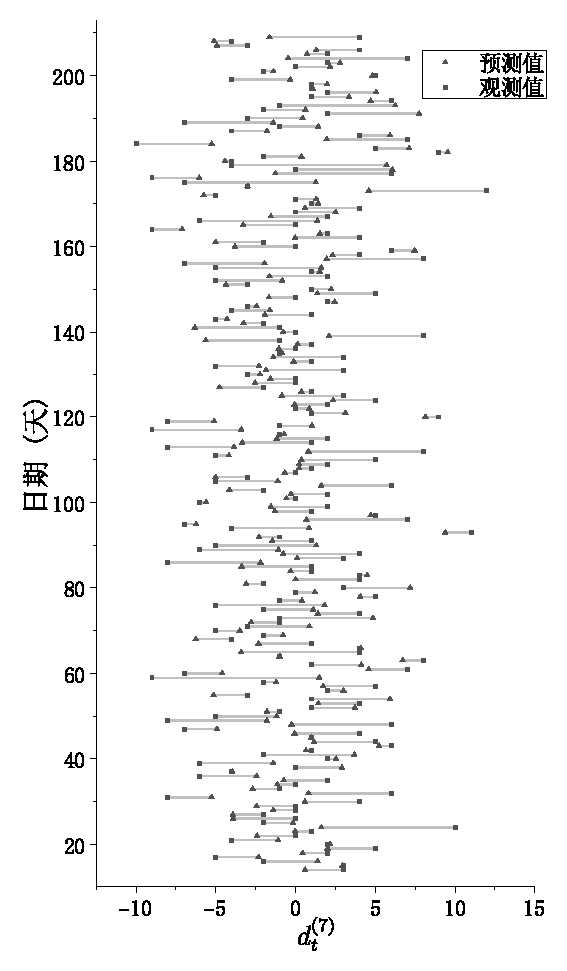
\includegraphics{Image/问题四展示.eps}
	\caption{时序预测效果}\label{时序预测效果}
\end{figure}

经过参数估计,原数据满足的递推关系已经得到,本文根据递推预报公式得到了第14天到第209天的预测值.
并与实际观测值一同绘入图7,在对应点间连线.
由图7可知,拟合趋势良好,数据间残差较小,满足预测需求,可以用于预报需求量.

\begin{figure}[!htbp]
	\centering
	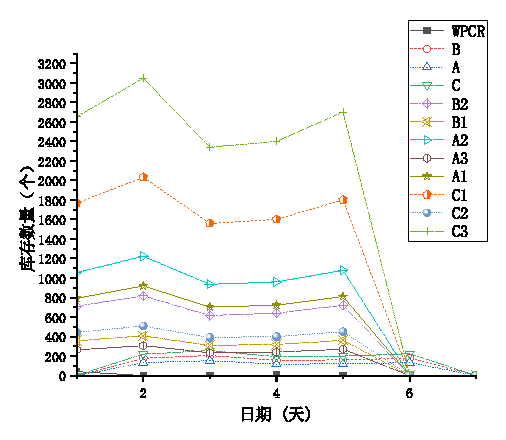
\includegraphics{Image/问题四库存.eps}
	\caption{预测每日库存}\label{预测每日库存}
\end{figure}

由图可知,工厂产量明显较大,足以保证正常交货.
但当需求量较少时,也会导致极大地浪费,这是由于未将概率计入目标函数导致的,可以再进一步改进.

% subsection 模型的求解 (end)
% subsection 模型的建立 (end)
% section _问题四_ (end)
